

\section{JavaScript}

\subsection{JS-Grundlagen}
\begin{code}{Web-Konsole}
    In JS mit dem Keyword \texttt{console}:
    \begin{itemize}
        \item \texttt{console.log(message)}: Loggt eine Nachricht
        \item \texttt{console.clear()}: Löscht die Konsole
        \item \texttt{console.trace(message)}: Stack trace ausgeben
        \item \texttt{console.error(message)}: stderr ausgeben
        \item \texttt{console.time()}: Startet einen Timer
        \item \texttt{console.timeEnd()}: Stoppt den Timer
    \end{itemize}
    Website für Konsolen-API: \url{https://nodejs.org/api/console.html}
\end{code}

\begin{definition}{Datentypen}
    
    Bekannte Datentypen wie bei Java, spezielle Datentypen:
    \begin{itemize}
        \item \texttt{undefined}: Variable wurde deklariert, aber nicht initialisiert
        \item \texttt{null}: Variable wurde deklariert und initialisiert, aber nicht belegt
        \item \texttt{Symbol}: Eindeutiger, unveränderlicher Wert
        \item \texttt{Number}: Ganze Zahlen, Fließkommazahlen, NaN, Infinity
        \begin{itemize}
            \item Infinity: $1/0$, $-1/0$
            \item NaN: $0/0$, $\sqrt{-1}$
        \end{itemize}
        \item \texttt{BigInt}: Ganze Zahlen beliebiger Größe
        \item \texttt{Object}: Sammlung von Schlüssel-Wert-Paaren
        \item \texttt{Function}: Funktionen sind Objekte
    \end{itemize}
    mit dem Keyword \texttt{typeof} kann der Datentyp zurückgegeben werden
\end{definition}

\begin{center}
    \begin{tabular}{lll}
    \hline
    typeof 12 & // & 'number' \\
    typeof(12) & // 'number' &  \\
    typeof 2 n & // & 'bigint' \\
    typeof Infinity & // 'number' &  \\
    typeof NaN & // 'number' !! &  \\
    typeof 'number' & // 'string' &  \\
    \hline
    \end{tabular}
\end{center}

\begin{concept}{Variablen Definition}
    \begin{itemize}
        \item \texttt{var}: Global oder lokal
        \item \texttt{let}: Nur lokal
        \item \texttt{const}: Konstante
    \end{itemize}
\end{concept}

\begin{definition}{Variablenbindung}
    \begin{itemize}
        \item \texttt{var}: Funktionsbindung
        \item \texttt{let}: Blockbindung
        \item \texttt{const}: Blockbindung
    \end{itemize}
    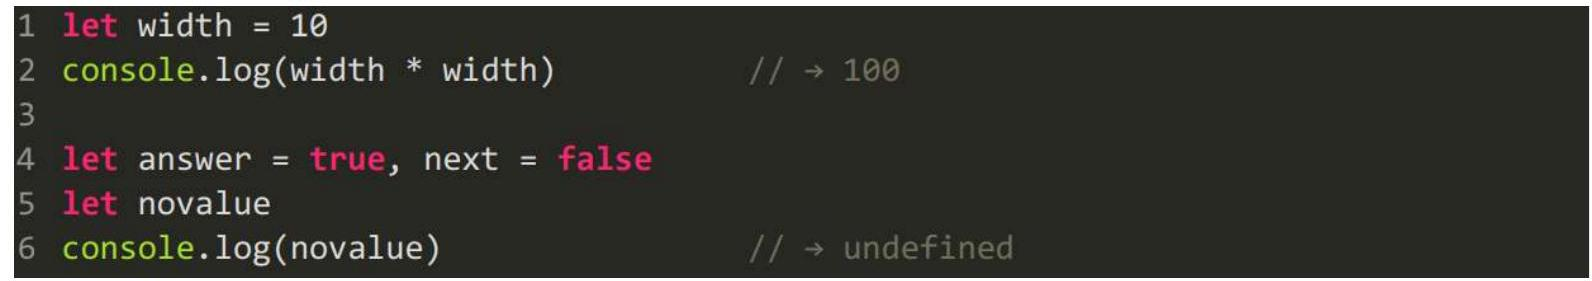
\includegraphics[width=\linewidth]{images/2024_12_29_858f09cde51177c71657g-05}
\end{definition}

\begin{definition}{Operatoren}
    \begin{itemize}
        \item Arithmetische Operatoren: $+, -, *, /, \%, ++, --$
        \item Zuweisungsoperatoren: $=, +=, -=, *=, /=, \%=, **=, <<=, >>=, >>>=, \&=, ^=, |=$
        \item Vergleichsoperatoren: $==, ===, !=, !==, >, <, >=, <=$
        \item Logische Operatoren: $\&\&, ||, !$
        \item Bitweise Operatoren: $\&, |, ^, ~, <<, >>, >>>$
        \item Sonstige Operatoren: \texttt{typeof}, \texttt{instanceof}
    \end{itemize}
\end{definition}

\begin{formula}{Vergleich mit \texttt{==} und \texttt{===}}
    \begin{itemize}
        \item \texttt{==}: Vergleicht Werte, konvertiert Datentypen
        \item \texttt{===}: Vergleicht Werte und Datentypen ohne Konvertierung
    \end{itemize}
    ebenfalls: \texttt{!=} und \texttt{!==}
\end{formula}

\begin{code}{Verzweigungen\text{,} Wiederholung und Switch Case}
    \begin{itemize}
        \item \texttt{if (condition) \{...\} else \{...\}}
        \item \texttt{switch (expression) \{ case x: ... break; default: ... \}}
        \item \texttt{for (initialization; condition; increment) \{...\}}
        \item \texttt{while (condition) \{...\}}
        \item \texttt{do \{...\} while (condition)}
        \item \texttt{for (let x of iterable) \{...\}}
    \end{itemize}
\end{code}

\begin{verbatim}
switch (<ausdruck>) {
    case <wert1>:
    break
    default:
        ...
        break
}
\end{verbatim}

\begin{verbatim}
if (<ausdruck>) \{
\} else \{
\end{verbatim}

\}

\begin{verbatim}
for (let i=1; i<50; i*=2) {
    console.log(i)
}
4 // -> 1, -> 2, -> 4, > 8, > 16, -> 32
\end{verbatim}

\begin{code}{Funktionsdefinition}
    \begin{itemize}
        \item \texttt{function name(parameters) \{...\}}
        \item \texttt{const name = (parameters) => \{...\}}
        \item \texttt{const name = parameters => \{...\}}
        \item \texttt{const name = parameters => expression}
    \end{itemize}
\end{code}

\begin{verbatim}
1 const square = function (x) {
    return x * x
}
4
5 console.log(square(12)) // -> 144
\end{verbatim}

\begin{verbatim}
1 const square1 $=(x) \Rightarrow$ \{return $x * x$ \}
2 const square2 $=x=x^{*} x$
\end{verbatim}

%\begin{example}
\begin{lstlisting}[language=JavaScript, style=base]
// Beispiel einer Funktion
function add(a, b) {
return a + b;
}
// Beispiel einer Arrow-Funktion
const add = (a, b) => a + b;
\end{lstlisting}
%\end{example}

\subsection{Objekte und Arrays}

\begin{concept}{Objekt vs Array}
    \begin{tabular}{|l|l|l|}
        \hline
        Was & Objekt & Array \\
        \hline
        Art & Attribut-Wert-Paare & Sequenz von Werten \\
        \hline
        Literalnotation & werte $=\{$ a: 1, b: 2$\}$ & liste $=[1,2,3]$ \\
        \hline
        Ohne Inhalt & werte $=\{ \}$ & liste $=[]$ \\
        \hline
        Elementzugriff & werte["a" $]$ oder werte.a & liste[0] \\
        \hline
        \end{tabular}
\end{concept}

\begin{definition}{Objekte}
    \begin{itemize}
        \item Objekt Attribute sind dynamisch und können einfach erweitert werden:
        \item Objekt Attribute können auch einfach mit dem delete keyword entfernt werden.
        \item Mit in kann überprüft werden, ob ein Attribut existiert
    \end{itemize}
\end{definition}


\begin{verbatim}
let person = {
    name: "John Baker",
    age: 23,
    "exam results": [5.5, 5.0, 5.0, 6.0, 4.5]
}
\end{verbatim}

\begin{verbatim}
    let obj = { message: "not yet implemented" }
    obj.ready = false
> obj
{ message: 'not yet implemented', ready: false }
> obj.attr
undefined
\end{verbatim}

\begin{verbatim}
> let obj = { message: "ready", ready: true, tasks: 3 }
> delete obj.message
> obj.tasks = undefined
> obj
{ ready: true, tasks: undefined }
> "message" in obj
false
> "tasks" in obj
true
\end{verbatim}

\begin{definition}{Methoden}
    Ein Objekt kann auch Methoden enthalten:
\end{definition}

\begin{verbatim}
> let cat = { type: "cat", sayHello: () => "Meow" }
> cat.sayHello
[Function: sayHello]
    > cat.sayHello()
'Meow'
\end{verbatim}

\begin{code}{Arrays}

    Verschiedene Hilfsfunktionen:

    \begin{itemize}
        \item Array.isArray()
        \item .push()
        \item .pop()
        \item Indexof, lastIndexOf
        \item Concat
        \item slice
        \item Shift, unshift
        \item .forEach(item => ....)
        \item .filter(item => .....)
        \item .map(item => ...)
    \end{itemize}

    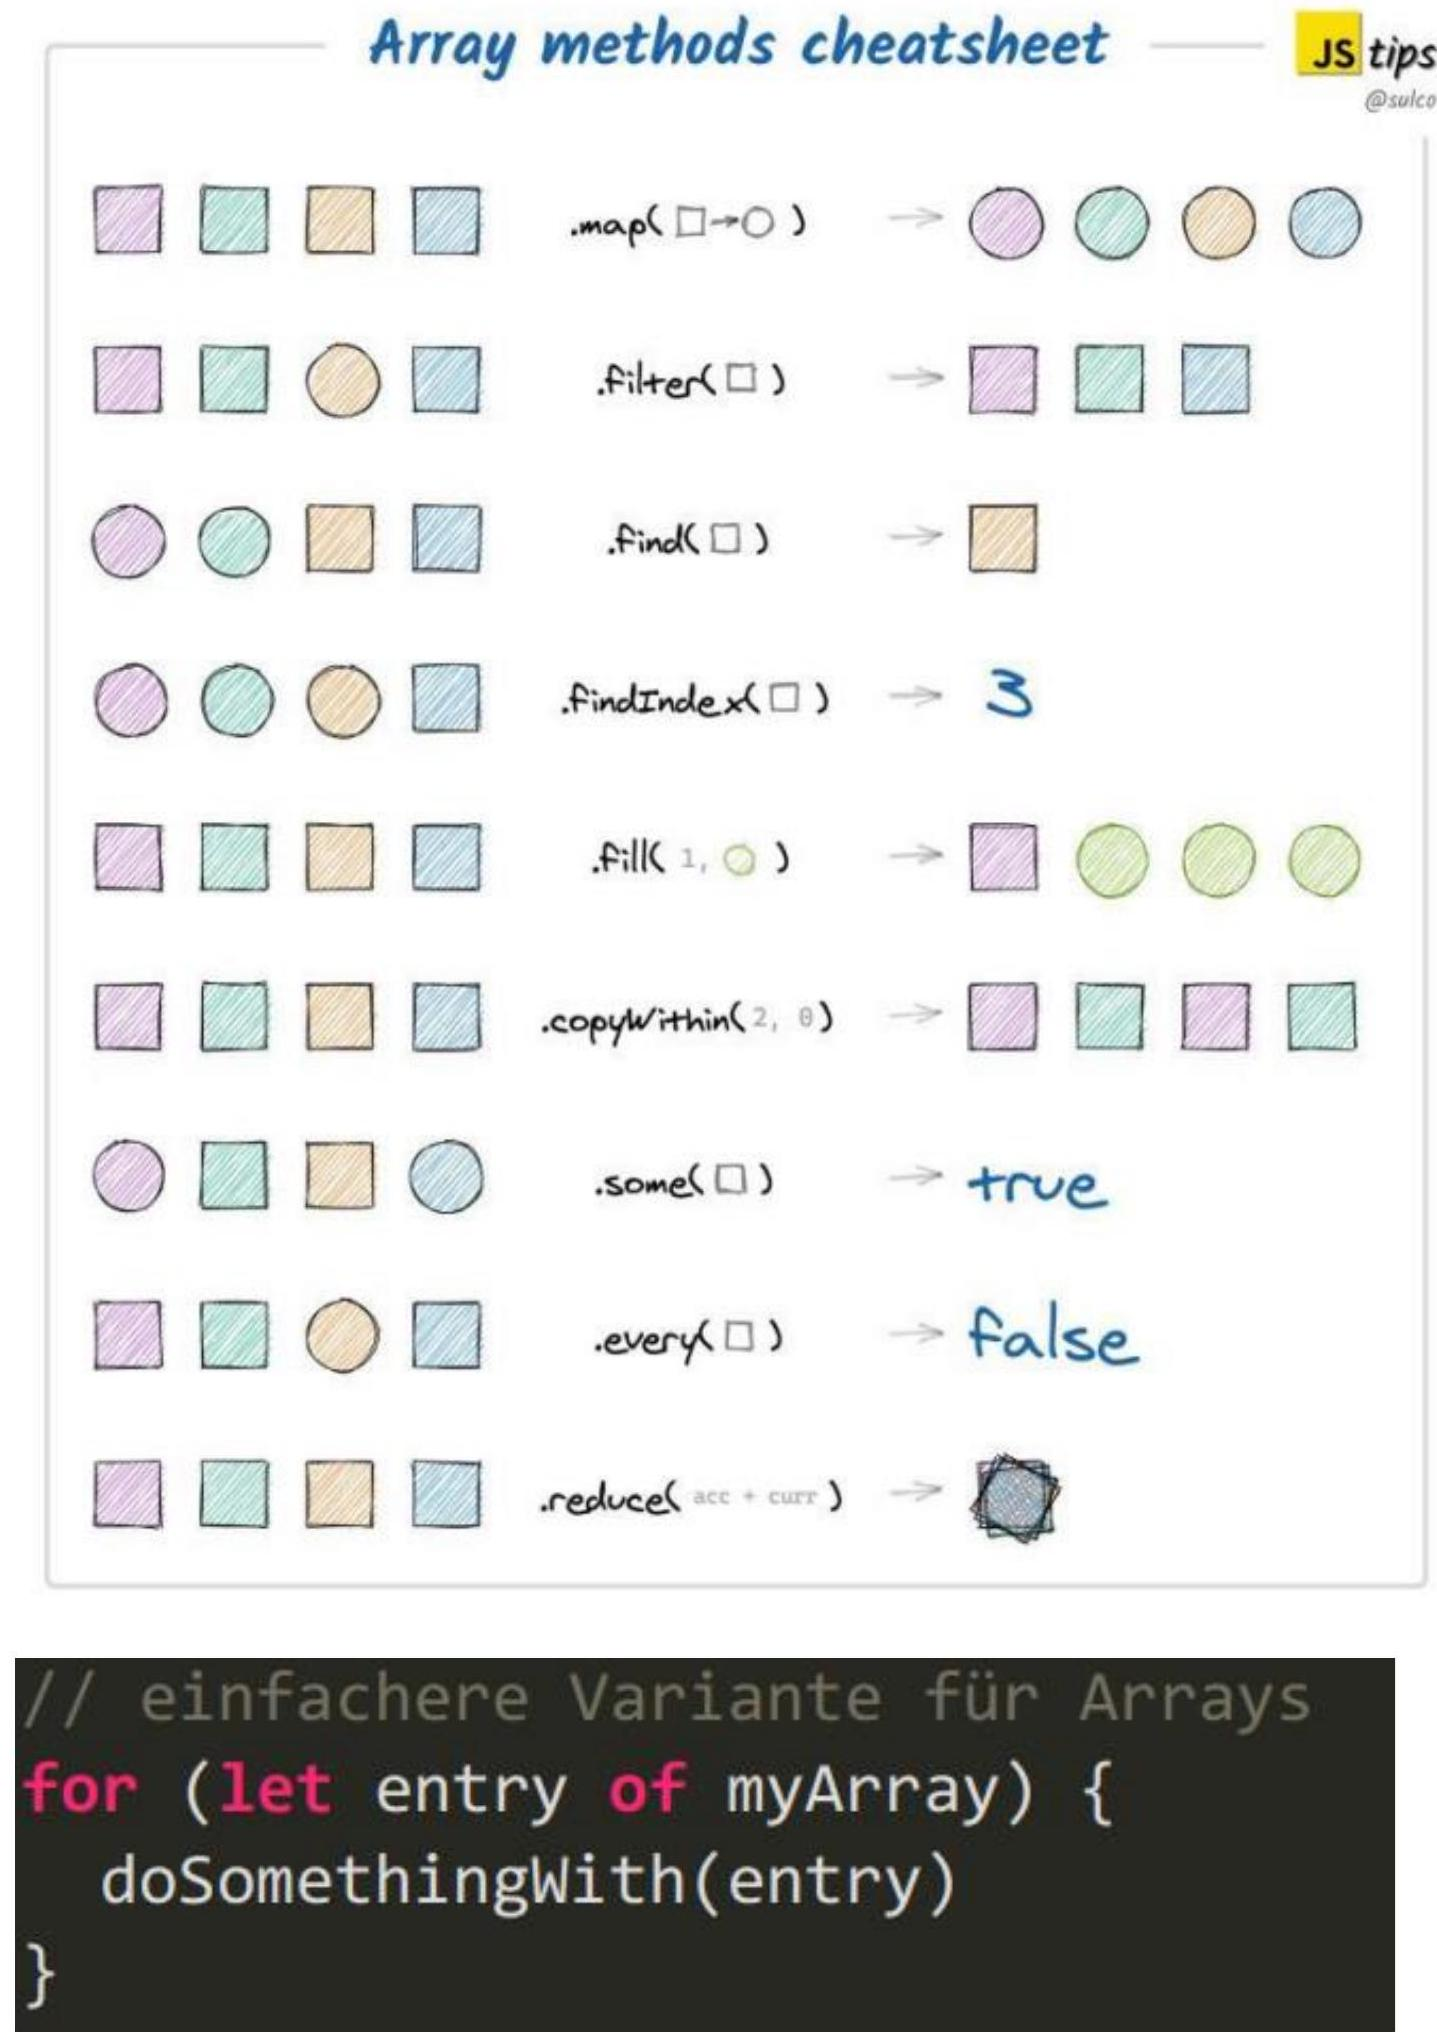
\includegraphics[width=\linewidth]{images/2024_12_29_858f09cde51177c71657g-08}
\end{code}

begin{concept}{Json: JavaScript Object Notation}
\begin{itemize}
    \item Daten-Austauschformat, nicht nur für JavaScript
    \item Orientiert an Notation für JavaScript-Objektliterale
  \end{itemize}
  https://www.json.org/json-en.html
\end{concept}
  
  \begin{verbatim}
  > JSON.stringify({ type: "cat", name: "Mimi", age: 3})
  '{"type":"cat", "name":"Mimi", "age":3}'
  > JSON.parse('{"type":"cat","name":"Mimi","age":3}')
  { type: 'cat', name: 'Mimi', age: 3 }
  \end{verbatim}


\subsection{Funktionen und funktionale Programmierung}

\begin{definition}{Funktionen}
    \begin{itemize}
        \item Funktionen sind spezielle, aufrufbare Objekte
        \item Man kann ihnen jederzeit Attribute oder Methoden hinzufügen
        \item Sie haben bereits vordefinierte Methoden
      \end{itemize}
\end{definition}

\begin{verbatim}
    const add = (x, y) => x + y
    add.doc = "This function adds two values"
        add(3,4)
    7
        add.doc
    'This function adds two values'
\end{verbatim}

\begin{concept}{Modulsystem in JavaScript}
    \begin{itemize}
        \item \texttt{import} und \texttt{export} für Module
        \item \texttt{export default} für Standardexport
        \item \texttt{import \{name\} from 'module'} für benannte Exports
        \item \texttt{import * as name from 'module'} für alle Exports
    \end{itemize}
\end{concept}

\begin{verbatim}
    1 /* car-lib.js */
    2}\mathrm{ const car = {
    3 brand: 'Ford',
    4 model: 'Fiesta'
    5 }
    6
    7 module.exports = car
    1 /* other js file */
    2 const car = require('./car-lib')
\end{verbatim}

\subsection{Prototypen von Objekten}

\begin{definition}{Prototypen}
    \begin{itemize}
        \item Die meisten Objekte haben ein Prototyp-Objekt.
        \item Dieses fungiert als Fallback für Attribute und Methoden.
      \end{itemize}
\end{definition}

\begin{verbatim}
    > Object.getPrototypeOf(Math.max) == Function.prototype
    true
    > Object.getPrototypeOf([]) == Array.prototype
    true
    > Object.getPrototypeOf(Function.prototype) == Object.prototype
    true
    > Object.getPrototypeOf(Array.prototype) == Object.prototype
    true
\end{verbatim}

\begin{code}{Prototypen-Kette}
    \begin{verbatim}
        function Employee (name, salary) {
            Person.call(this, name)
            this.salary = salary
        }
        Employee.prototype = new Person()
        Employee.prototype.constructor = Employee
        let e17 = new Employee("Mary", 7000)
        console.log(e17.toString()) /* -> Person with name 'Mary' */
        console.log(e17.salary) /* -> 7000 */
        \end{verbatim}
        
        Call, apply, bind
        
        \begin{itemize}
          \item Weitere Argumente von call : Argumente der Funktion
          \item Weiteres Argument von apply : Array mit den Argumenten
          \item Erzeugt neue Funktion mit gebundenem this
        \end{itemize}
\end{code}

\begin{code}{Klassen}
    \begin{itemize}
        \item Klassen sind syntaktischer Zucker für Prototypen
        \item Klassen können Attribute und Methoden enthalten
        \item Klassen können von anderen Klassen erben
    \end{itemize}

    \begin{verbatim}
        class Person {
            constructor (name) {
                this.name = name
            }
            toString () {
                return `Person with name '${this.name}'
            }
        }
        let p35 = new Person("John")
        console.log(p35.toString()) // -> Person with name 'John'
        \end{verbatim}
\end{code}

\begin{code}{Vererbung}
    \begin{verbatim}
        class Employee extends Person {
            constructor (name, salary) {
                super(name)
                this.salary = salary
            }
            toString () {
                return `${super.toString()} and salary ${this.salary}
            }
        }
        let e17 = new Employee("Mary", 7000);
        console.log(e17.toString()) /* -> Person with name 'Mary' and salary 7000 */
        console.log(e17.salary) /* -> 7000 */
        \end{verbatim}
\end{code}

\begin{code}{Getter und Setter}
    \begin{verbatim}
        class PartTimeEmployee extends Employee {
            constructor (name, salary, percentage) {
                super(name, salary)
                this.percentage = percentage
            }
            get salary100 () { return this.salary * 100 / this.percentage}
            set salary100 (amount) { this.salary = amount * this.percentage / 100 }
        }
        let e18 = new PartTimeEmployee("Bob", 4000, 50)
        console.log(e18.salary100) /* -> 8000 */
        e18.salary100 = 9000
        console.log(e18.salary) /* \ 4500 */
        \end{verbatim}
\end{code}

\subsection{Asynchrone Programmierung}

\subsection{Webserver}